\documentclass[a4paper]{report}
\usepackage[utf8]{inputenc}
\usepackage[portuguese]{babel}
\usepackage{hyperref}
\usepackage{a4wide}
\hypersetup{pdftitle={TP2:  Protocolo IPv4  (Parte I)},
pdfauthor={João Teixeira, José Ferreira, Miguel Solino},
colorlinks=true,
urlcolor=blue,
linkcolor=black}
\usepackage{subcaption}
\usepackage[cache=false]{minted}
\usepackage{listings}
\usepackage{booktabs}
\usepackage{multirow}
\usepackage{appendix}
\usepackage{tikz}
\usepackage{authblk}
\usepackage{bashful}
\usepackage{verbatim}
\usepackage{amsmath}
\usetikzlibrary{positioning,automata,decorations.markings}
\AfterEndEnvironment{figure}{\noindent\ignorespaces}

\begin{document}

\title{TP2:  Protocolo IP (Parte I e II)\\ 
\large Grupo Nº 7}
\author{João Teixeira (A85504) \and José Ferreira (A83683) \and Miguel Solino (A86435)}

\date{\today}

\begin{center}
    \begin{minipage}{0.75\linewidth}
        \centering
        
\includegraphics[width=0.4\textwidth]{images/eng.jpeg}\par\vspace{1cm}
        \vspace{1cm}
        \href{https://www.uminho.pt/PT}
        {\color{black}{\scshape\LARGE Universidade do Minho}} \par
        \vspace{1cm}
        \href{https://www.di.uminho.pt/}
        {\color{black}{\scshape\Large Departamento de Informática}} \par
        \maketitle
    \end{minipage}
\end{center}

\tableofcontents

\pagebreak
\chapter{Parte 1}
\section{Exercício 1}

\begin{figure}[H]
    \centering 
    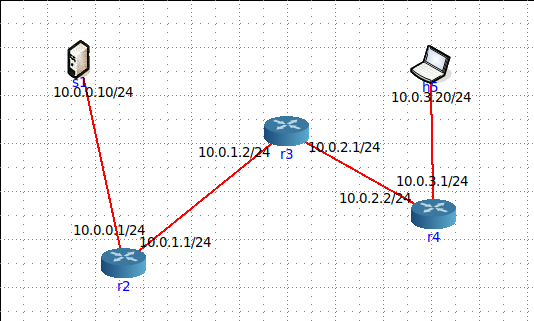
\includegraphics[width=\textwidth]{images/coreEx1.png}  
    \caption{Ex. 1 - Core}
    \label{fig:coreEx1}
\end{figure}

\subsection{Alínea a}
\textbf{Active o wireshark ou o tcpdump no pc s1. Numa shell de s1, execute o
comando traceroute -l para o endereço IP do host h5.}

\begin{figure}[H]
    \centering 
    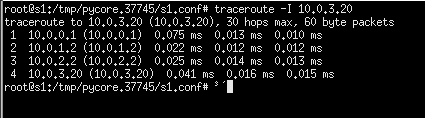
\includegraphics[width=\textwidth]{images/traceroutEx1.png}  
    \caption{Ex. 1 - Traceroute}
    \label{fig:traceroutEx1}
\end{figure}
\subsection{Alínea b}
\textbf{Registe e analise o tráfego ICMP enviado enviado por s1 e tráfego ICMP
recebido como resposta. Comente os resultados face ao comportamento esperado.}\\
Analisando os resultados obtidos, constatamos que o envio de pacotes teve duas
fases.\\
As fases estão divididas entre os pacotes com TTL abaixo de 4 e os com TTL acima
de 4.\\
Na primeira fase, os pacotes com TTL = 1, TTL = 2 e TTL = 3 foram descartados
pelos routers r1, r2 e r3, respetivamente. Para cada um destes foi recebido um
pacote \textit{Time-to-live exceeded}.\\
Na segunda fase, ao contrário dos pacotes anteriores, nenhum deles foi
descartado tendo como resposta pacotes \textit{Echo (ping) reply}.

\begin{figure}[H]
    \centering 
    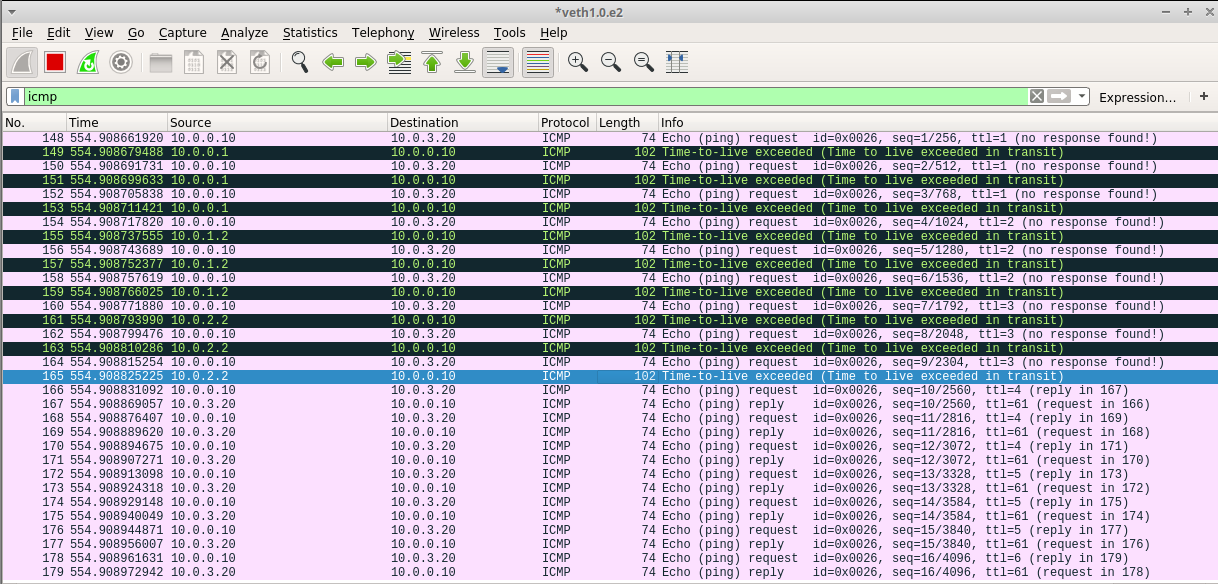
\includegraphics[width=\textwidth]{images/wiresharkEx1.png}  
    \caption{Ex. 1 - Wireshark}
    \label{fig:wiresharkEx1}
\end{figure}
\subsection{Alínea c}
\textbf{Qual deve ser o valor inicial mínimo do campo TTL para alcançar o
destino h5? Verifique na prática que a sua resposta está correta.}\\
Face aos resultados analisados na questão anterior, verifica-se que a partir de
TTL = 4 os pacotes deixam de receber mensagem de erro como resposta, logo o
valor inicial mínimo para alcançar o destino h5 deverá ser 4.

\subsection{Alínea d}
\textbf{Qual o valor médio do tempo de ida-e-volta (Round-Trip Time) obtido?}\\
\begin{math}
RTT = ((0.075 + 0.013 + 0.010) / 3 + (0.022 + 0.012 + 0.012) / 3 + (0.025 +
0.014 + 0.013) / 3 + (0.041 + 0.016 + 0.015) / 3) * 2 = 0.178
\end{math}

\section{Exercício 2}

\begin{figure}[H]
    \centering 
    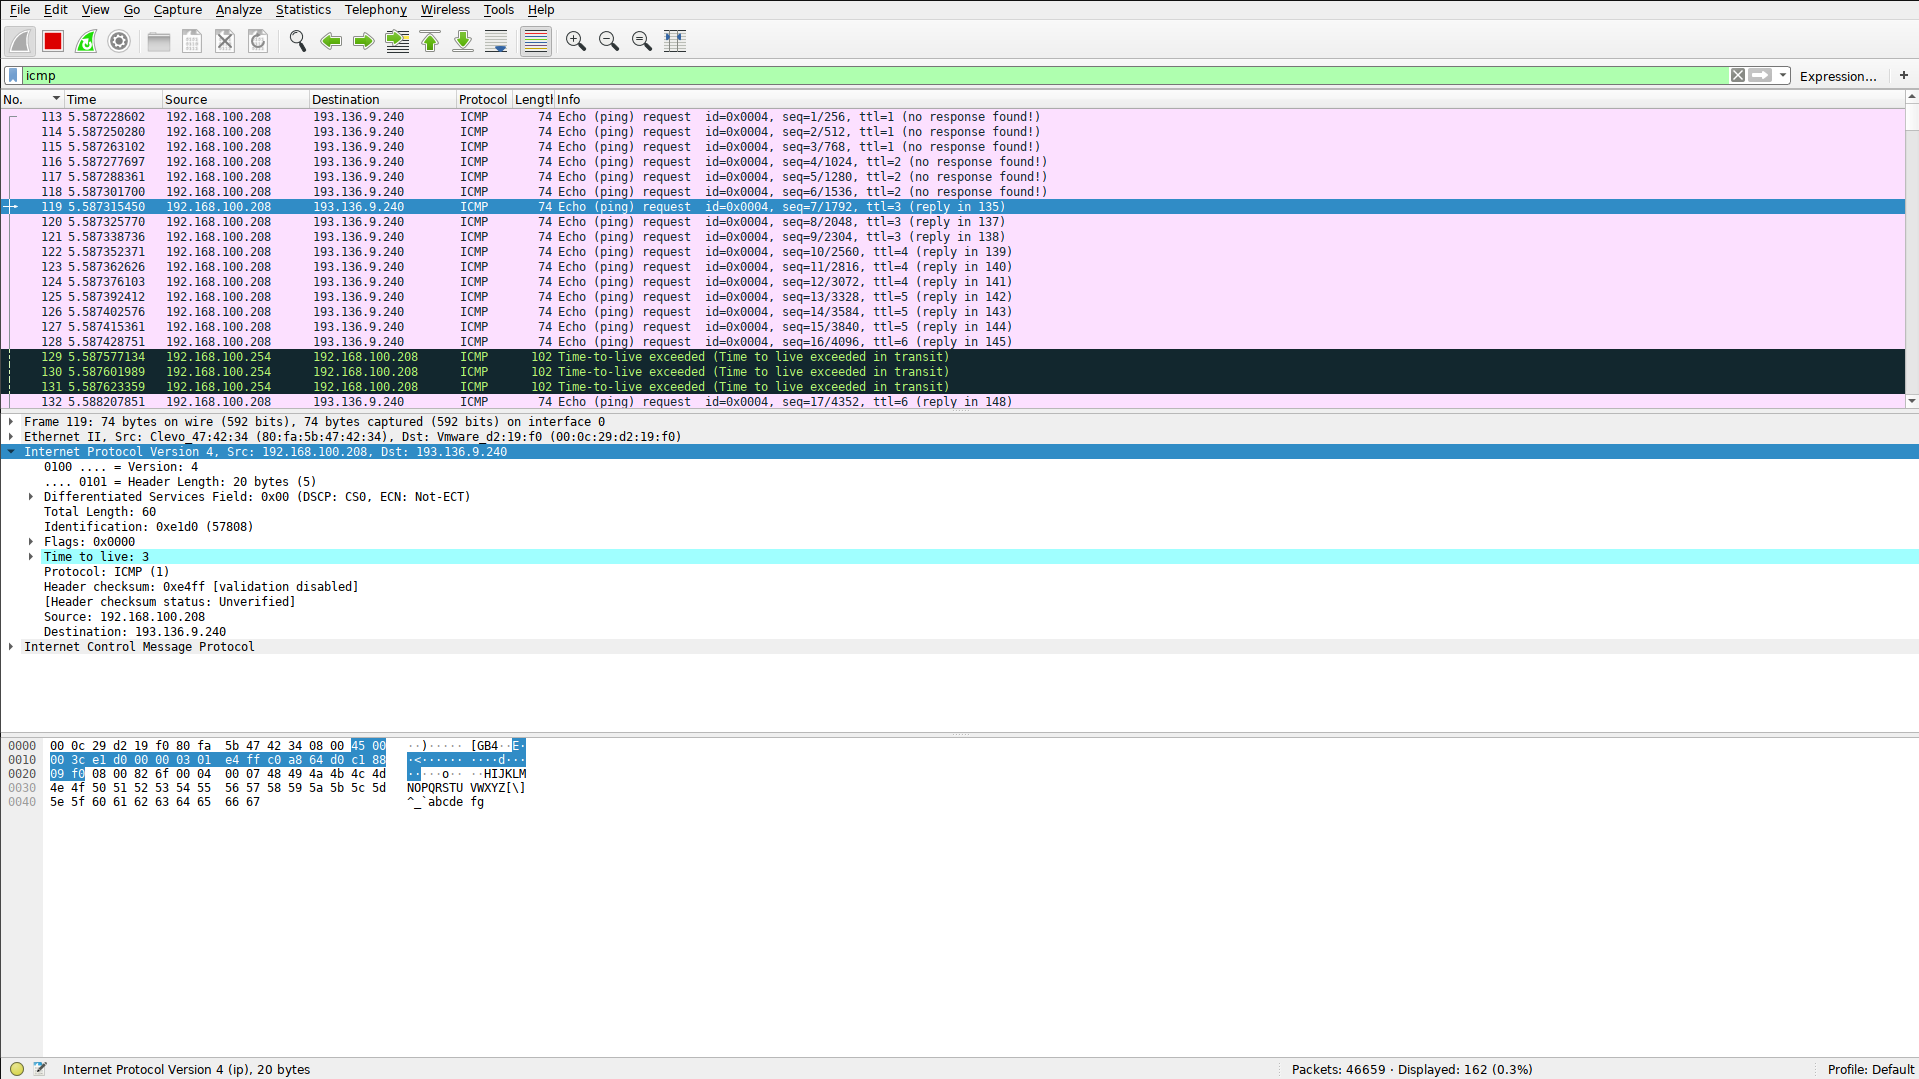
\includegraphics[width=\textwidth]{images/wiresharkEx2.png}  
    \caption{Ex. 2 - Wireshark}
    \label{fig:wiresharkEx2}
\end{figure}

\subsection{Alínea a}
\textbf{Qual é o endereço IP da interface ativa do seu computador?}
\begin{figure}[H]
    \centering 
    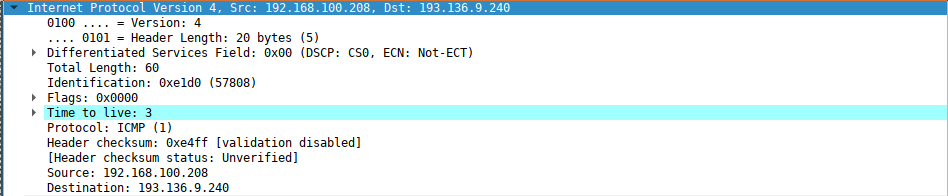
\includegraphics[width=\textwidth]{images/ipEx2.png}
    \caption{Ex. 2 - Cabeçalho IP}
    \label{fig:ipEx2}
\end{figure}
192.168.100.208

\subsection{Alínea b}
\textbf{Qual é o valor do campo protocolo? O que identifica?}\\
ICMP (1).\\
O valor do campo protocolo é 1, ou seja, identifica o protocolo ICMP.

\subsection{Alínea c}
\textbf{Quantos bytes tem o cabeçalho IP(v4)? Quantos bytes tem o
campo de dados (payload) do datagrama? Como se calcula o tamanho 
do payload?}\\
O cabeçalho IP tem 20 bytes, analisando o campo Header length na 
figura \ref{fig:ipEx2}.\\
O tamanho do campo de dados (payload) é a diferença entre o número 
total de bytes e o tamanho do cabeçalho do datagrama:\\
Payload = 60 - 20 = 40 bytes.

\subsection{Alínea d}
\textbf{O datagrama IP foi fragmentado? }

\begin{figure}[H]
    \centering 
    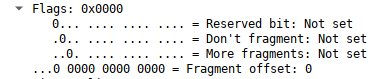
\includegraphics[width=\textwidth]{images/ipEx2Flags.png}
    \caption{Ex. 2 - Flags do Cabeçalho IP}
    \label{fig:ipEx2Flags}
\end{figure}
Observando a figura \ref{fig:ipEx2Flags} reparamos que no 
campo Flags, tudo está a 0, logo o \textit{Fragment offset} tem valor 0, o que
Tendo em atenção agora a flag \textit{More Fragments} concluímos que não existem
mais fragmentos pois, se o valor for 1 existem, caso contrário é 0. Logo,
se estamos no primeiro fragmento e não existem mais então este é o datagrama
original.

\subsection{Alínea e}
\textbf{Ordene os pacotes capturados de acordo com o endereço IP 
fonte (e.g., selecionando o cabeçalho
da coluna Source), e analise a sequência de tráfego ICMP gerado a partir 
do endereço IP atribuído à interface da sua máquina. Para a sequência 
de mensagens ICMP enviadas pelo seu computador, indique que campos do 
cabeçalho IP variam de pacote para pacote.}\\
Após ordenarmos, concluímos que os campos do cabeçalho IP que variam de 
pacote para pacote são o \textit{TTL}, \textit{Header Checksum} e o
identificador.

\begin{figure}[H]
    \centering 
    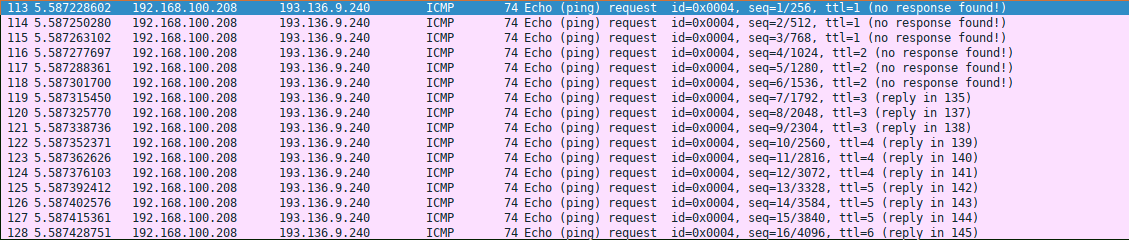
\includegraphics[width=\textwidth]{images/wiresharkSourceEx2.png}
    \caption{Ex. 2 - Tráfego Wireshark ordenado por endereço fonte}
    \label{fig:wiresharkSourceEx2}
\end{figure}
\subsection{Alínea f}
\textbf{Observa algum padrão nos valores do campo de Identificação do datagrama
IP e TTL?}\\
Ao analisar o datagrama IP, verificamos que este conserva os primeiros 8 bits em
todos o casos apresentados e os restantes são incrementados sequencialmente.\\
Também observamos que o TTL é incrementado sequencialmente

\subsection{Alínea g}
\textbf{Ordene o tráfego capturado por endereço destino e encontre a 
série de repostas ICMP TTL exceeded enviadas ao seu computador. Qual é o
valor do campo TTL? Esse valor permanece constante para todas as mensagens 
de resposta ICMP TTL exceed enviados ao seu host? Porquê?}\\
O valor do campo TTL é 62.\\
Para todas as mensagens de resposta ICMP TTL exceeded recebidas no nosso host
esse valor manteve-se constante. O TTL mostrado (predefinido pelo destino) é 64.
No entanto, no final, quando o pacote chega ao destino é 61, devido a ter
passado por 2 routers antes de chegar, sendo então decrementado 2 vezes.

\begin{figure}[H]
    \centering 
    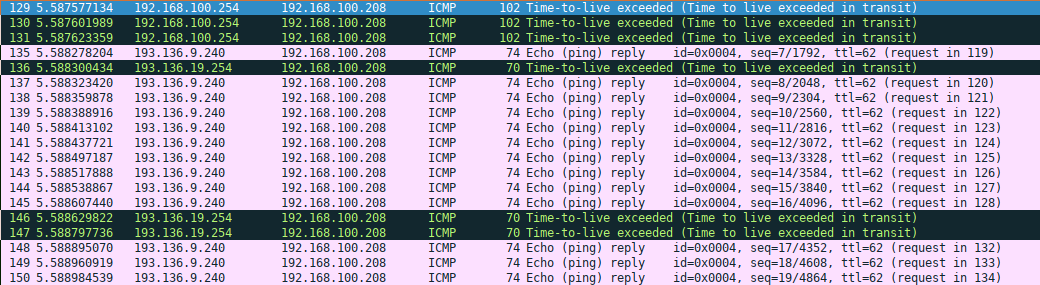
\includegraphics[width=\textwidth]{images/wiresharkDestinyEx2.png}
    \caption{Ex. 2 - Tráfego Wireshark ordenado por endereço de destino}
    \label{fig:wiresharkDestinyEx2}
\end{figure}

\section{Exercício 3}

\begin{figure}[H]
    \centering 
    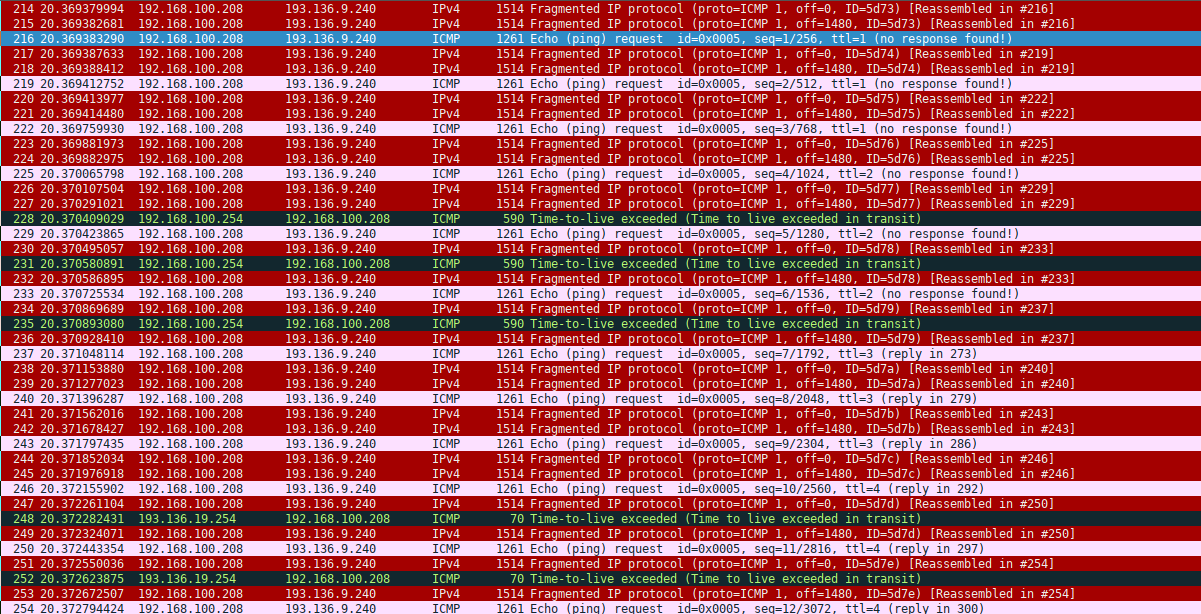
\includegraphics[width=\textwidth]{images/datagramaIpEx3.png}
    \caption{Ex.3 - Fragmentos do datagrama IP}
    \label{fig:datagramaIpEx3}
\end{figure}
\subsection{Alínea a}
\textbf{Localize a primeira mensagem ICMP. Porque é que houve 
necessidade de fragmentar o pacote inicial?}\\
Analisando a figura, vemos que a primeira mensagem ICMP é a 214.\\
Porque o tamanho permitido pelo protocolo é inferior ao tamanho do PDU, sendo
assim necessário ser fragmentado para ser possível circular na rede.

\subsection{Alínea b}
\textbf{Imprima o primeiro fragmento do datagrama IP segmentado. 
Que informação no cabeçalho IP indica que se trata do primeiro fragmento? 
Qual é o tamanho deste datagrama IP?}

\begin{figure}[H]
    \centering 
    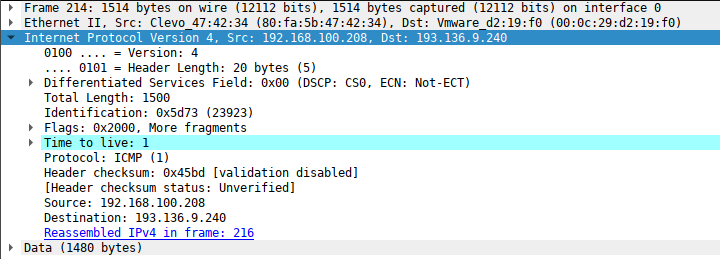
\includegraphics[width=\textwidth]{images/fragmentDatagramaIpEx3.png}
    \caption{Ex.3 - Cabeçalho do primeiro fragmento do datagrama IP}
    \label{fig:fragmentDatagramaIpEx3}
\end{figure}
Podemos observar na figura que, no campo Flags, o \textit{More fragments} tem
valor 1, isso indica que o diagrama foi fragmentado, existindo então mais
fragmentos.\\
Seguidamente, podemos ver que o \textit{Fragment offset} é 0, provando de que se
trata do primeiro fragmento.\\
A \textit{Total Length} e igual a 1500 bytes

\subsection{Alínea c}
\textbf{Imprima o segundo fragmento do datagrama IP original. Que
informação do cabeçalho IP indica que não se trata do 1º fragmento? 
Há mais fragmentos? O que nos permite afirmar isso?}

\begin{figure}[H]
    \centering 
    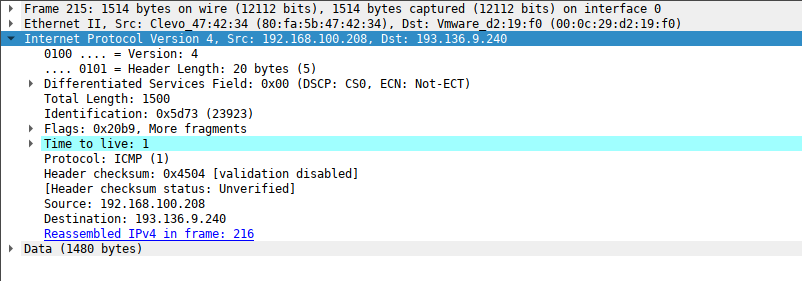
\includegraphics[width=\textwidth]{images/fragment2DatagramaIpEx3.png}
    \caption{Ex.3 - Cabeçalho do segundo fragmento do datagrama IP}
    \label{fig:fragment2DatagramaIpEx3}
\end{figure}
Para se verificar se um fragmento é o primeiro basta ter em atenção o valor
que está no \textit{Fragment offset}. Se esse valor for 0 então podemos concluir
que se trata do primeiro.\\
Sim, mais fragmentos existem porque o bit correspondente ao \textbf{More
fragments} é 1.

\subsection{Alínea d}
\textbf{Quantos fragmentos foram criados a partir do datagrama original?
Como se detecta o último fragmento correspondente ao datagrama original?}\\
Como está mostrado na imagem, o terceiro fragmento do datagrama original
tem o bit correspondente a \textit{More fragments} a 0, ou seja, não há mais 
fragmentos a seguir a este. Concluindo assim que foram criados 3 fragmentos 
(214, 215 e 216).

\subsection{Alínea e}
\textbf{Indique, resumindo, os campos que mudam no cabeçalho IP entre 
os diferentes fragmentos, e explique a forma como essa informação permite
reconstruir o datagrama original.}\\
Ao longo dos diferentes fragmentos, no cabeçalho IP, é alterado o
\textit{Fragment offset} e o \textit{More Fragments}. O primeiro permite
identificar a posição do fragmento no datagrama original, já o segundo, indica
se, além deste, existem mais fragmentos do datagrama original.


\chapter{Parte 2}

\begin{figure}[H]
    \centering 
    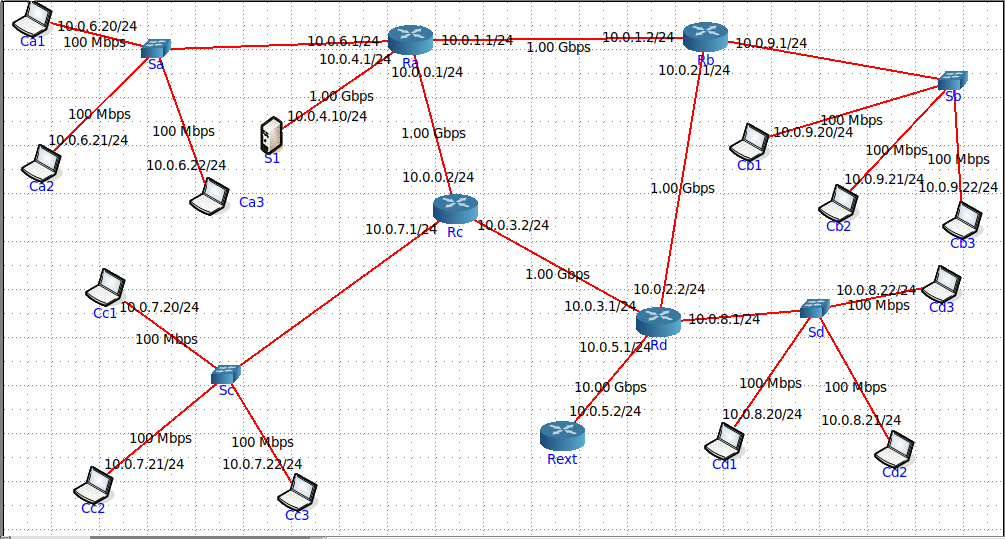
\includegraphics[width=\textwidth]{images/topologiaCore.png}
    \caption{Topologia Core}
    \label{fig:topologiaCore}
\end{figure}

\section{Exercício 1}

\subsection{Alínea a}
\textbf{Indique que endereços IP e máscaras de rede foram atribuídos pelo CORE a cada
equipamento. Para simplificar, pode incluir uma imagem que ilustre de forma clara a
topologia definida e o endereçamento usado.}

\subsection{Alínea b}
\textbf{Trata-se de endereços públicos ou privados? Porquê?}

\subsection{Alínea c}
\textbf{Por que razão não é atribuído um endereço IP aos switches?}

\subsection{Alínea d}
\textbf{Usando o comando ping certifique-se que existe conectividade IP entre 
os laptops dos vários departamentos e o servidor do departamento A 
(basta certificar-se da conectividade de um laptop por departamento).}

\begin{figure}[H]
    \centering 
    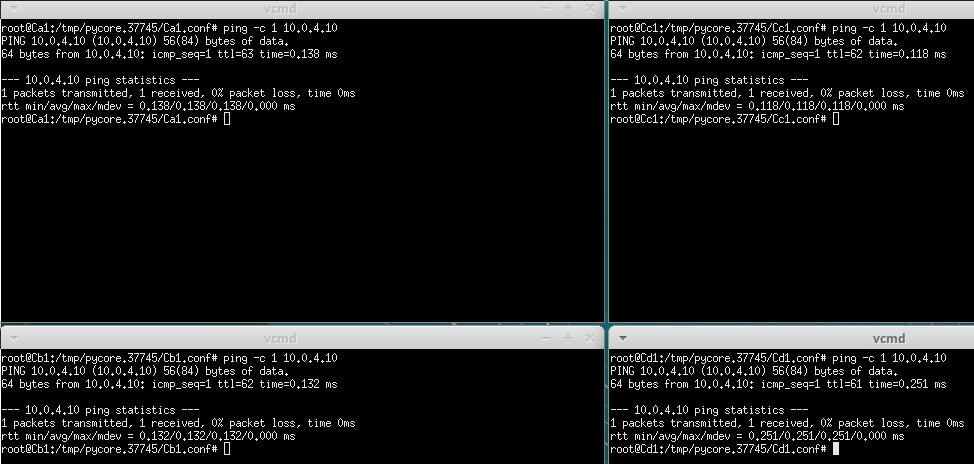
\includegraphics[width=\textwidth]{images/pingEx1P2.png}
    \caption{Ex.1 - Ping}
    \label{fig:pingEx1P2}
\end{figure}

\subsection{Alínea e}
\textbf{Verifique se existe conectividade IP do router de acesso Rext para o servidor S1.}

\begin{figure}[H]
    \centering 
    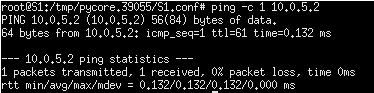
\includegraphics[width=\textwidth]{images/RextPing.png}
    \caption{Ex.2 - Conectividade Router Rext - S1}
    \label{fig:RextPing}
\end{figure}

\section{Exercício 2}

\subsection{Alínea a}
\textbf{Execute o comando netstat –rn por forma a poder consultar a tabela de
encaminhamento unicast (IPv4). Inclua no seu relatório as tabelas de encaminhamento
obtidas; interprete as várias entradas de cada tabela. Se necessário, consulte o manual
respetivo (man netstat).}

\begin{figure}[H]
    \centering 
    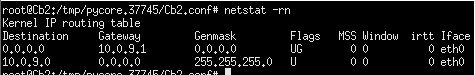
\includegraphics[width=\textwidth]{images/netstatPcEx2P2.png}
    \caption{Ex.2 - netstat pc departamento B}
    \label{fig:netstatPcEx2P2}
\end{figure}

\begin{figure}[H]
    \centering 
    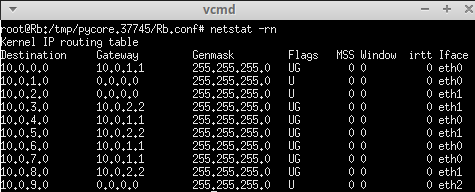
\includegraphics[width=\textwidth]{images/netstatRouterEx2P2.png}
    \caption{Ex.2 - netstat Router departamento B}
    \label{fig:netstatRouterEx2P2}
\end{figure}

\subsection{Alínea b}
\textbf{Diga, justificando, se está a ser usado encaminhamento estático ou dinâmico
(sugestão: analise que processos estão a correr em cada sistema).}

\begin{figure}[H]
    \centering 
    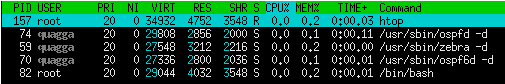
\includegraphics[width=\textwidth]{images/htop2a.png}
    \caption{Ex.2 - Processos a serem executados em Ra}
    \label{fig:htop2a}
\end{figure}

\begin{figure}[H]
    \centering 
    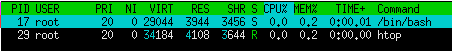
\includegraphics[width=\textwidth]{images/htopca1.png}
    \caption{Ex.2 - Processos a serem executados em Ca1}
    \label{fig:htopca1}
\end{figure}

\subsection{Alínea c}
\textbf{Admita que, por questões administrativas, a rota por defeito (0.0.0.0 ou 
default) deve ser retirada definitivamente da tabela de encaminhamento do 
servidor S1 localizado no departamento A. Use o comando route delete para o 
efeito. Que implicação tem esta medida para os utilizadores da empresa que 
acedem ao servidor? Justifique.}

\begin{figure}[H]
    \centering 
    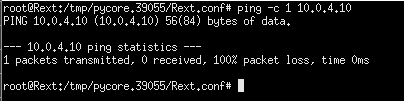
\includegraphics[width=\textwidth]{images/pingRextS1.png}
    \caption{Ex.2 - Ping do Rext para S1}
    \label{fig:pingRextS1}
\end{figure}

\begin{figure}[H]
    \centering 
    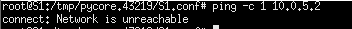
\includegraphics[width=\textwidth]{images/pingS1Rext.png}
    \caption{Ex.2 - Ping do S1 para Rext}
    \label{fig:pingS1Rext}
\end{figure}



\subsection{Alínea d}
\textbf{Adicione as rotas estáticas necessárias para restaurar a conectividade
para o servidor S1 por forma a contornar a restrição imposta na alínea c). Utilize
para o efeito o comando route add e registe os comandos que usou.}

\subsection{Alínea e}
\textbf{Teste a nova política de encaminhamento garantindo que o servidor está novamente
acessível utilizando para o efeito o comando ping. Registe a nova tabela de
encaminhamento do servidor.}

\section{Exercício 3}

\subsection{Alínea 1}
\textbf{Considere que dispõe apenas do endereço de rede IP 172.yyx.32.0/20, em que “yy”
são os dígitos correspondendo ao seu número de grupo (Gyy) e “x” é o dígito 
correspondente ao seu turno prático (PLx). Defina um novo esquema de endereçamento para 
as redes dos departamentos (mantendo a rede de acesso e core inalteradas) e atribua 
endereços às interfaces dos vários sistemas envolvidos. Deve justificar as opções usadas.}

\subsection{Alínea 2}
\textbf{Qual a máscara de rede que usou (em notação decimal)? Quantos interfaces IP pode 
interligar em cada departamento? Justifique.}

\subsection{Alínea 3}
\textbf{Garanta e verifique que a conectividade IP entre as várias redes locais da 
organização MIEI-RC é mantida. Explique como procedeu.}

\chapter{Conclusão}

\end{document}
